\documentclass[a4paper]{article}

\usepackage{amsmath}
\usepackage[english]{babel}
\usepackage[babel=true]{microtype}
\usepackage{wrapfig}
\usepackage{url}
\usepackage{mathrsfs} 
\usepackage[absolute]{textpos}
\usepackage{graphicx}
\usepackage{geometry}
\geometry{a4paper,left=40mm,right=30mm, top=3cm, bottom=3cm} 
\usepackage{subcaption}
\usepackage{float}

\newcommand{\Fermi}{\textit{Fermi} }

\begin{document}

\begin{figure}
    \begin{subfigure}{0.5\textwidth}
        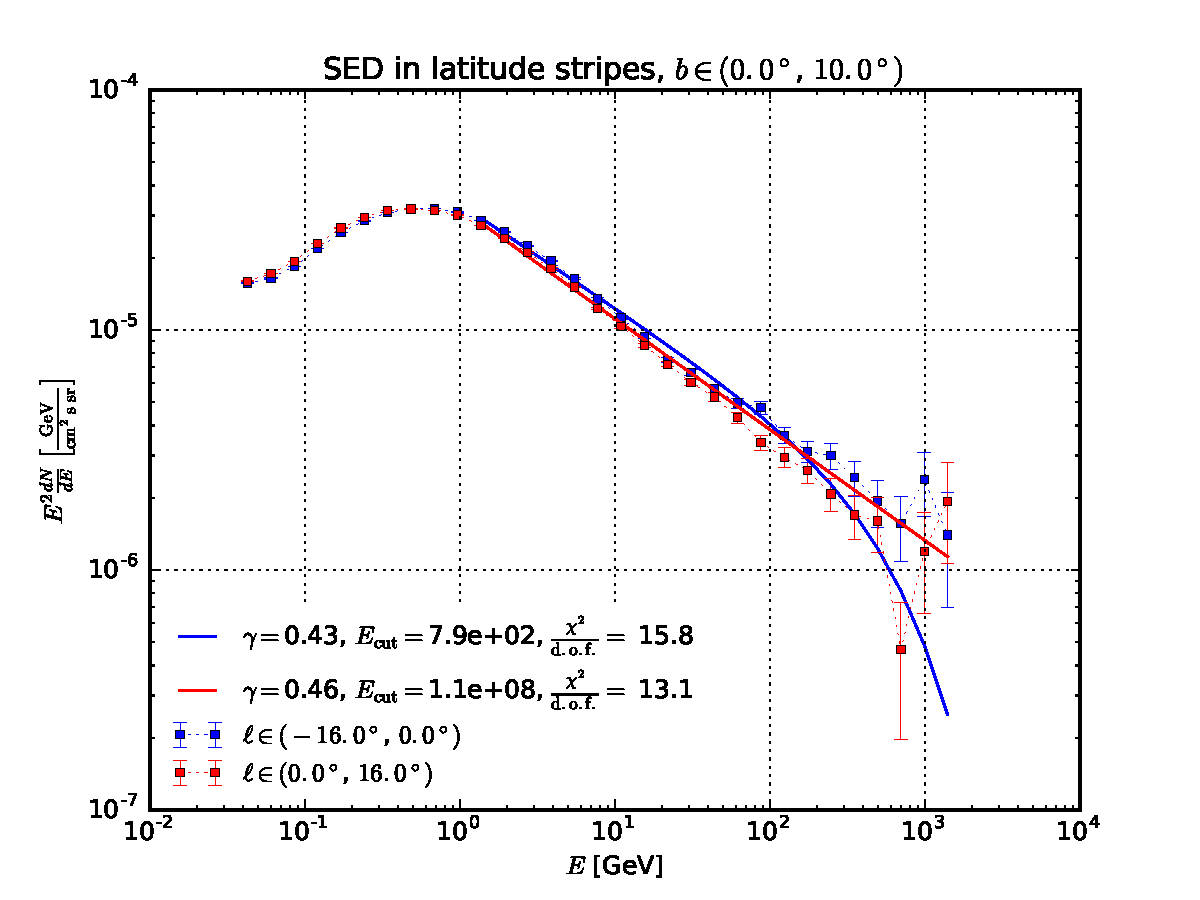
\includegraphics[width=\textwidth]{spectrum_of_top_bubble_in_lat_stripes_0-10.pdf}
    \end{subfigure} 
    \begin{subfigure}{0.5\textwidth}
        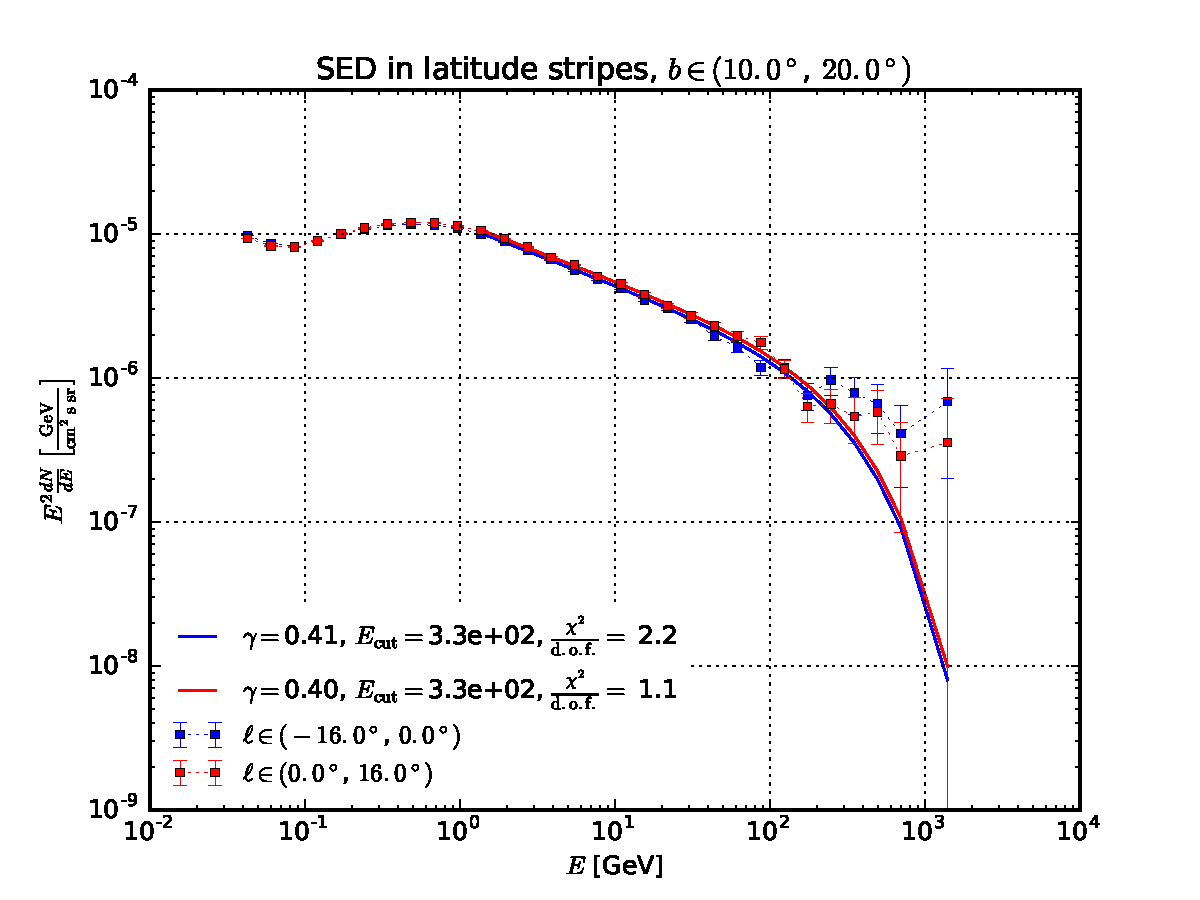
\includegraphics[width=\textwidth]{spectrum_of_top_bubble_in_lat_stripes_10-20.pdf}
    \end{subfigure}
    \begin{subfigure}{0.5\textwidth}
        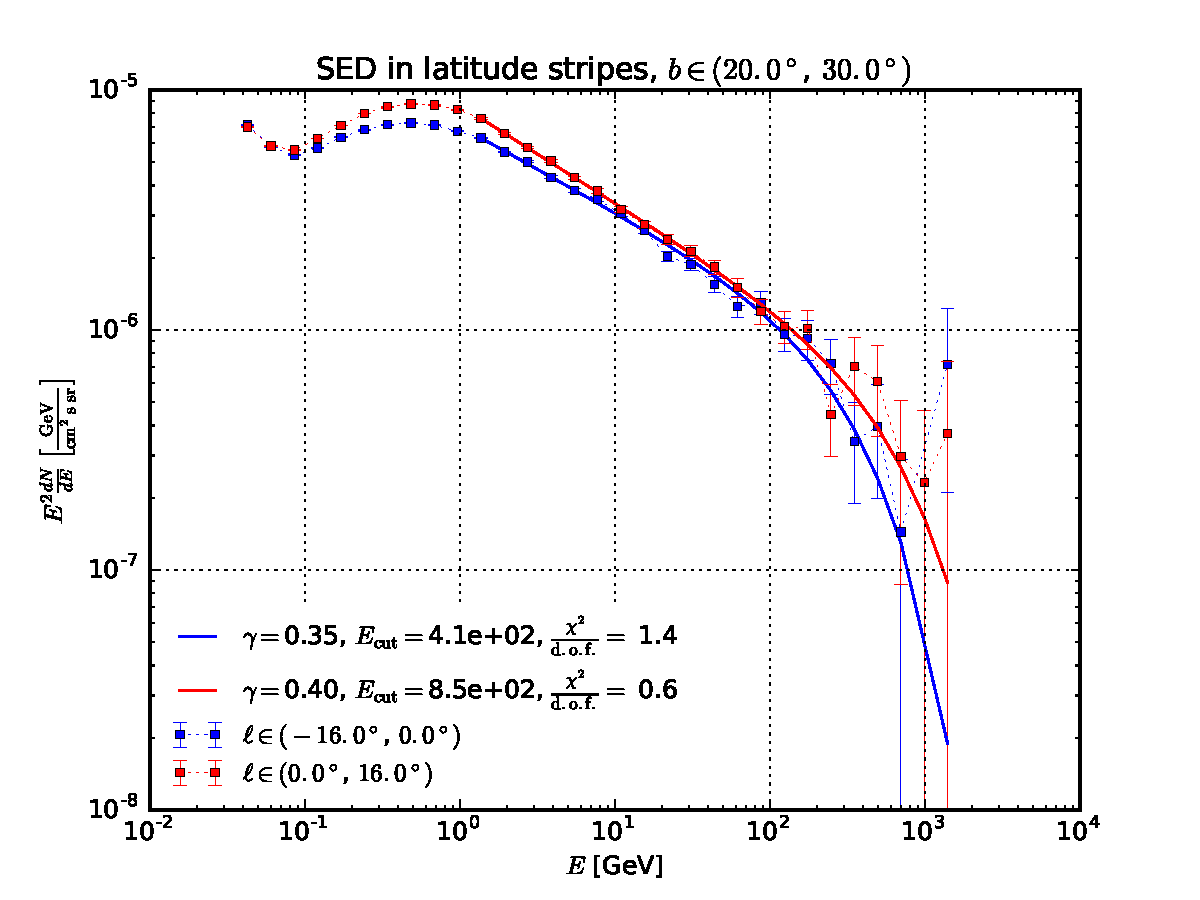
\includegraphics[width=\textwidth]{spectrum_of_top_bubble_in_lat_stripes_20-30.pdf}
    \end{subfigure} 
    \begin{subfigure}{0.5\textwidth}
        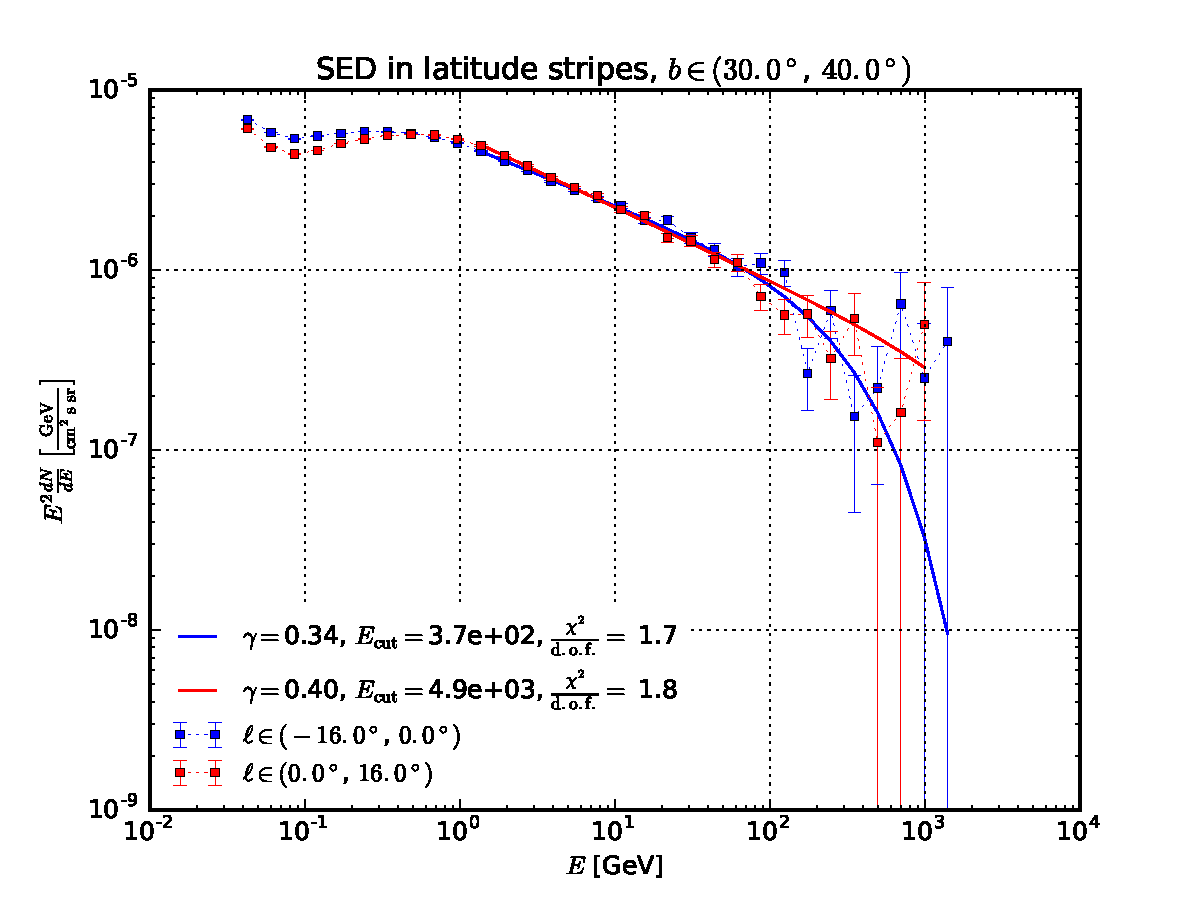
\includegraphics[width=\textwidth]{spectrum_of_top_bubble_in_lat_stripes_30-40.pdf}
    \end{subfigure}
    \begin{subfigure}{0.5\textwidth}
        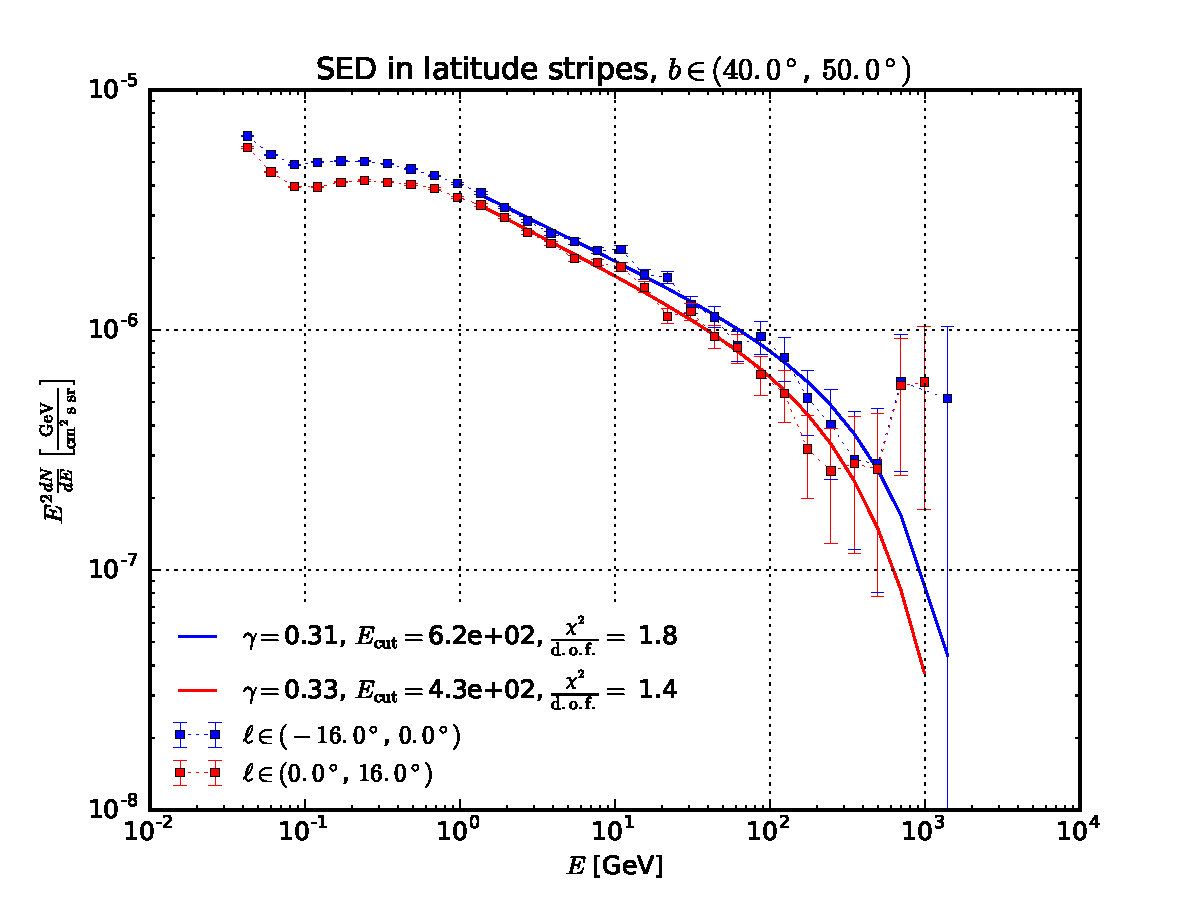
\includegraphics[width=\textwidth]{spectrum_of_top_bubble_in_lat_stripes_40-50.pdf}
    \end{subfigure} 
    \begin{subfigure}{0.5\textwidth}
        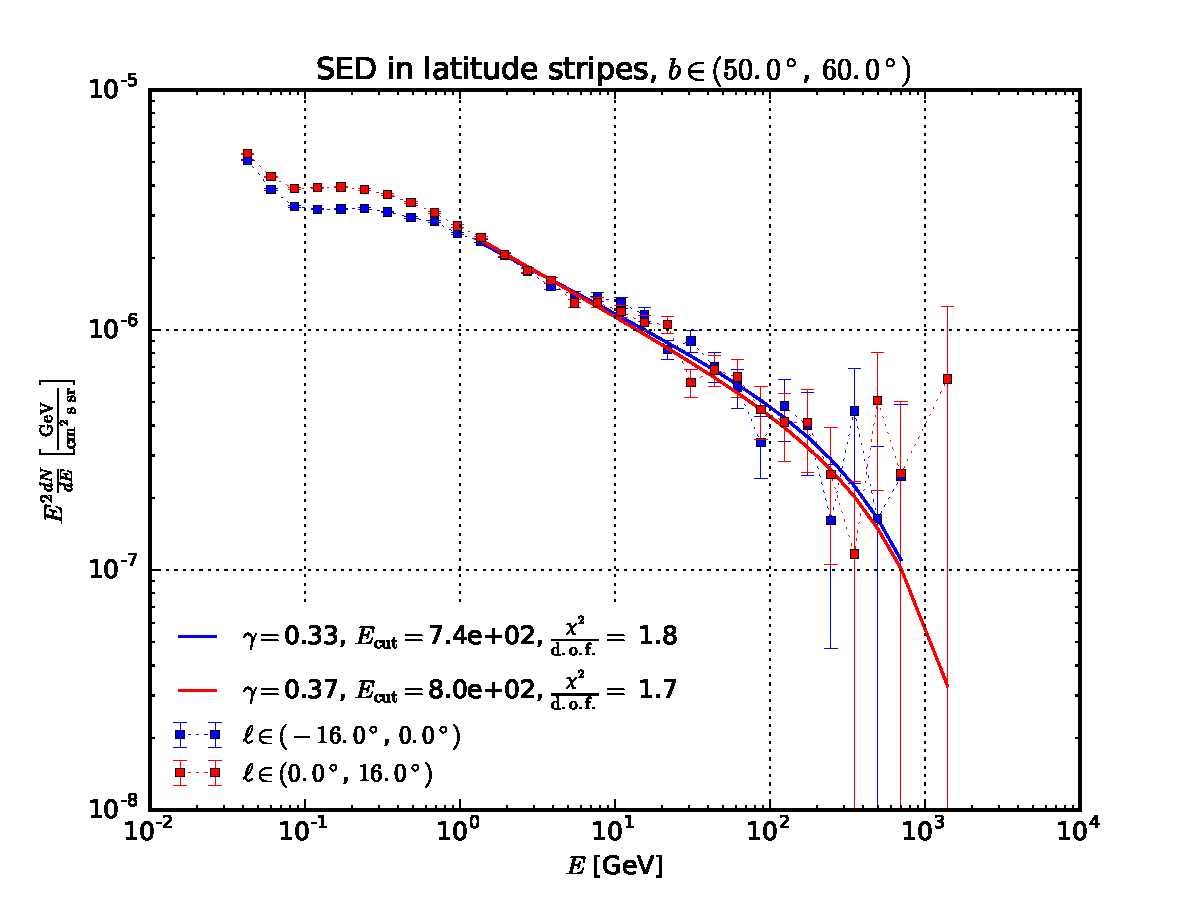
\includegraphics[width=\textwidth]{spectrum_of_top_bubble_in_lat_stripes_50-60.pdf}
    \end{subfigure}
    \caption{Spectral energy distribution of northern bubble (pure data) in $10^\circ$ latitude stripes. Point sources are masked. A powerlaw with cutoff is fitted to the data above 1 GeV. The western part of the bubble (blue) might have a little harder spectrum at most latitudes. When a powerlaw without cutoff is fitted, the spectral index of the western bubble is harder in almost every latitude stripe on the northern hemisphere. However, the difference is tiny. Only at low latitudes, $b \in (0^\circ, 10^\circ)$, the difference becomes visible. Maybe the fraction of the emission coming from the bubbles is too low.}
\end{figure}

\begin{figure}
    \begin{subfigure}{0.5\textwidth}
        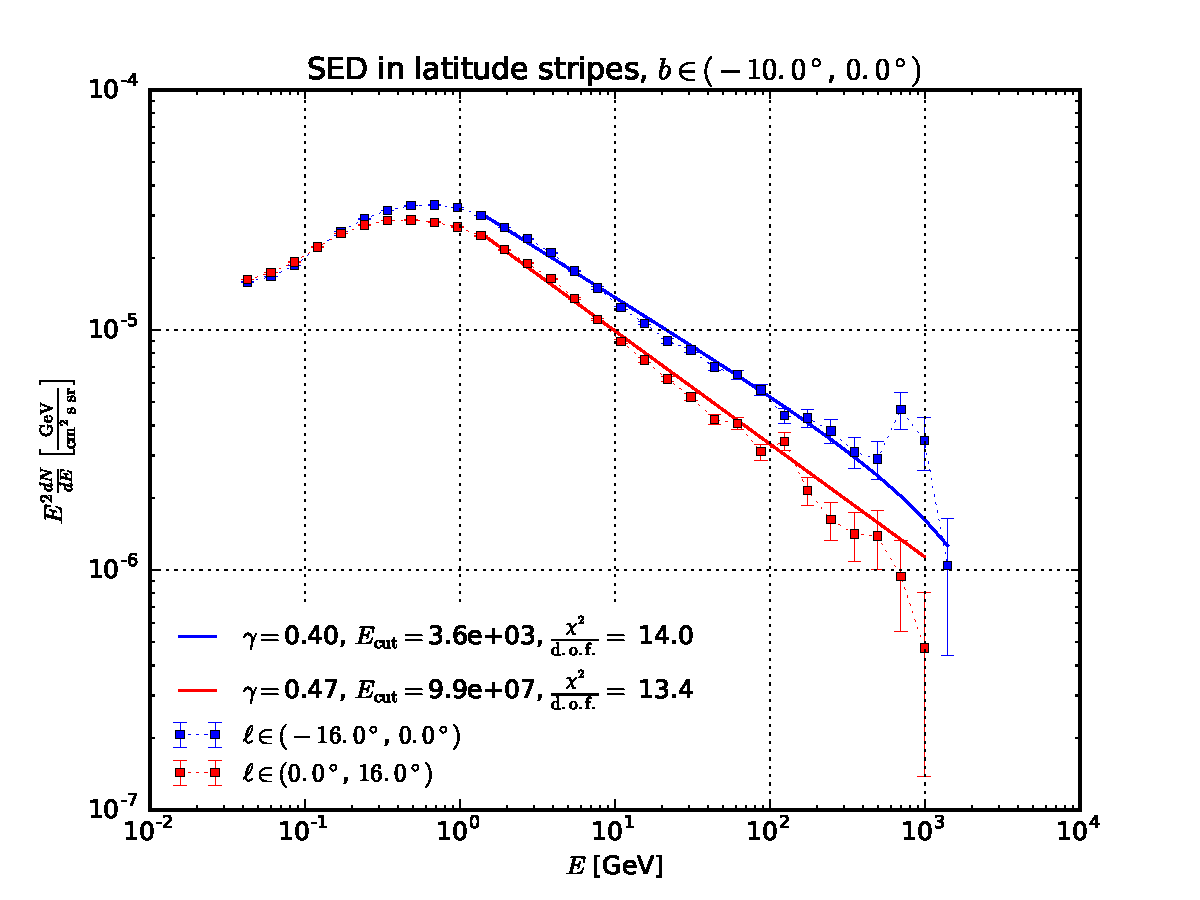
\includegraphics[width=\textwidth]{spectrum_of_bottom_bubble_in_lat_stripes_0-10.pdf}
    \end{subfigure} 
    \begin{subfigure}{0.5\textwidth}
        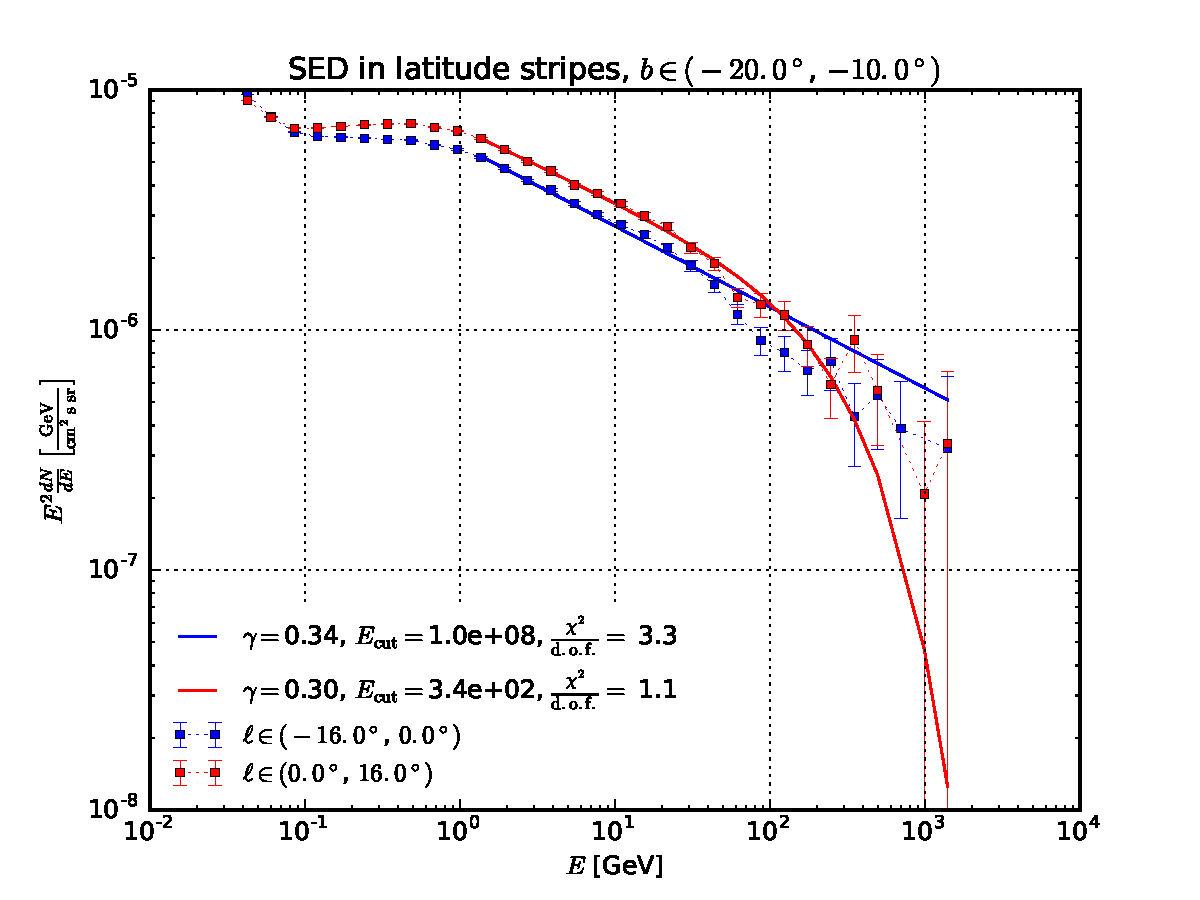
\includegraphics[width=\textwidth]{spectrum_of_bottom_bubble_in_lat_stripes_10-20.pdf}
    \end{subfigure}
    \begin{subfigure}{0.5\textwidth}
        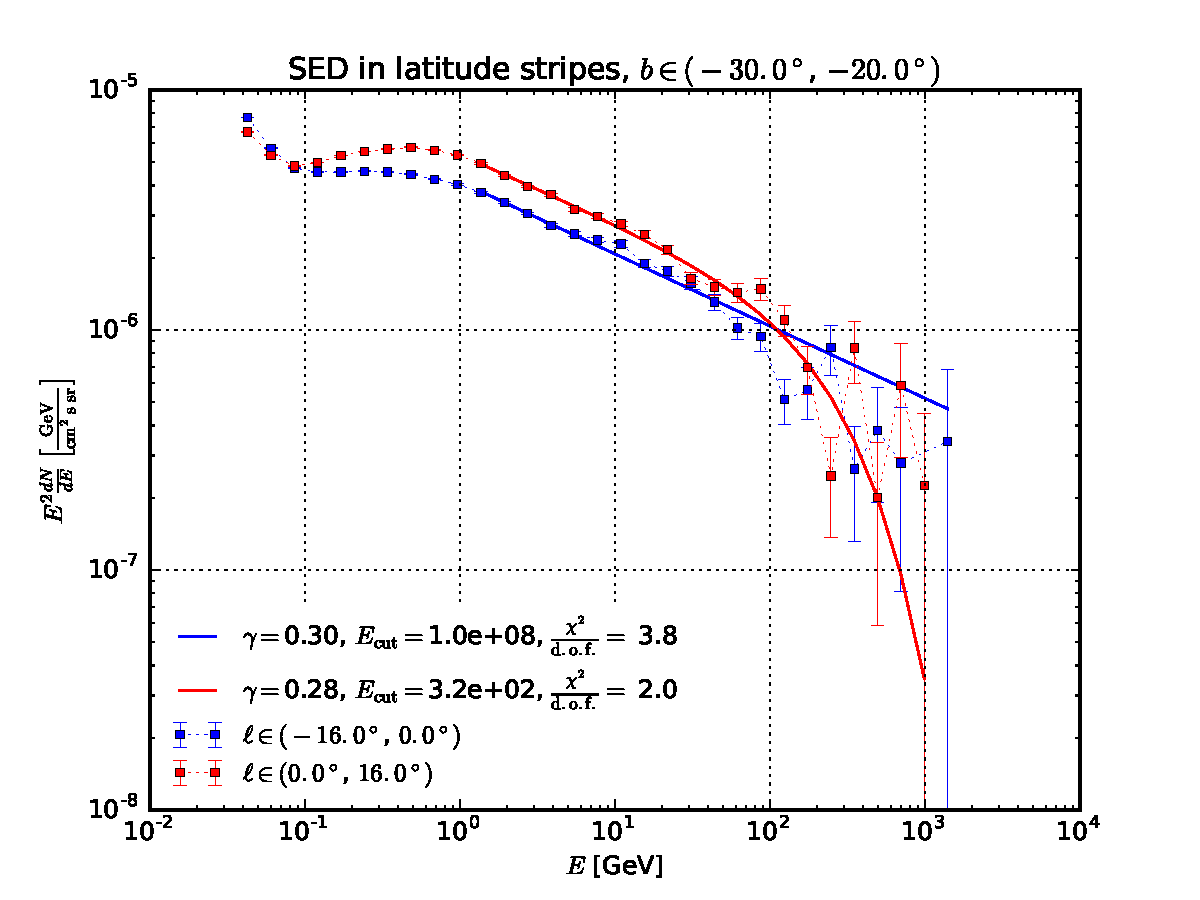
\includegraphics[width=\textwidth]{spectrum_of_bottom_bubble_in_lat_stripes_20-30.pdf}
    \end{subfigure} 
    \begin{subfigure}{0.5\textwidth}
        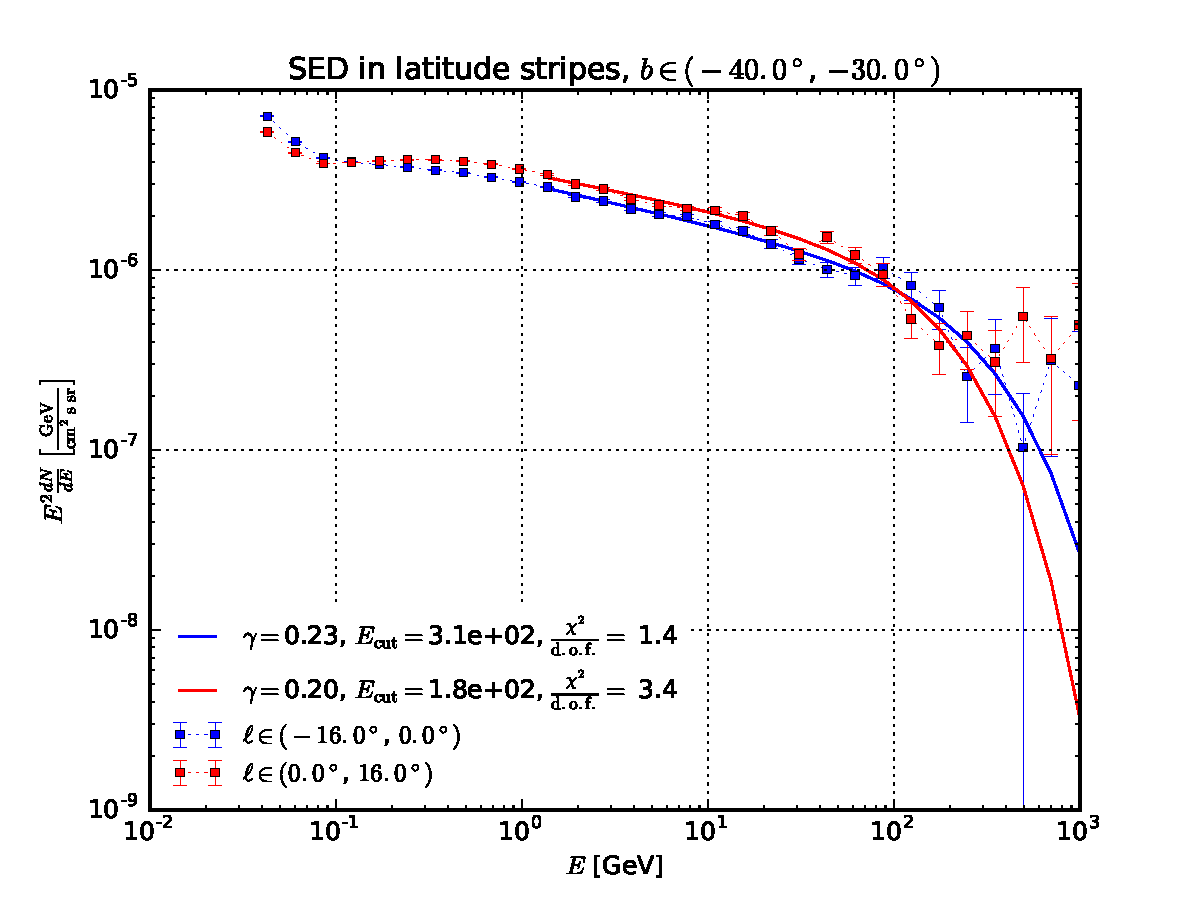
\includegraphics[width=\textwidth]{spectrum_of_bottom_bubble_in_lat_stripes_30-40.pdf}
    \end{subfigure}
    \begin{subfigure}{0.5\textwidth}
        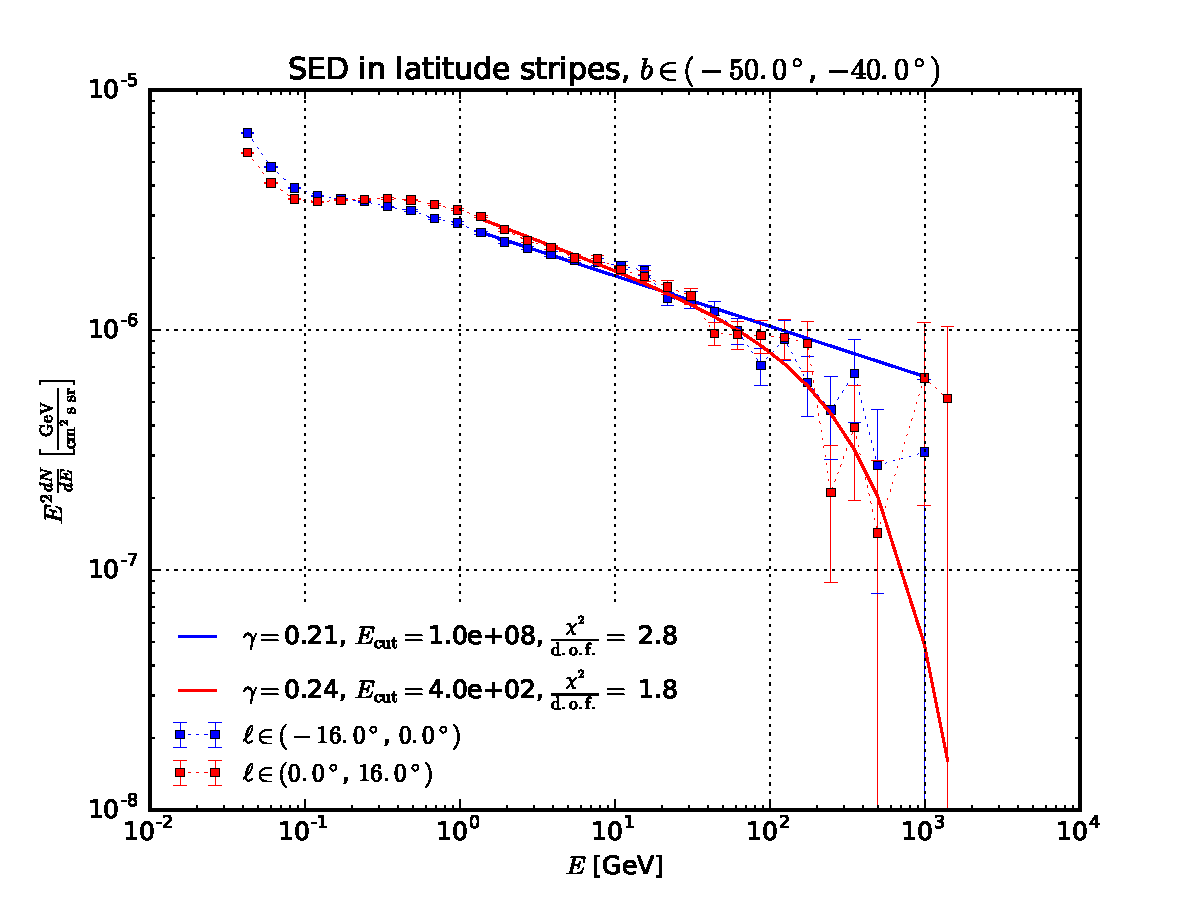
\includegraphics[width=\textwidth]{spectrum_of_bottom_bubble_in_lat_stripes_40-50.pdf}
    \end{subfigure} 
    \begin{subfigure}{0.5\textwidth}
        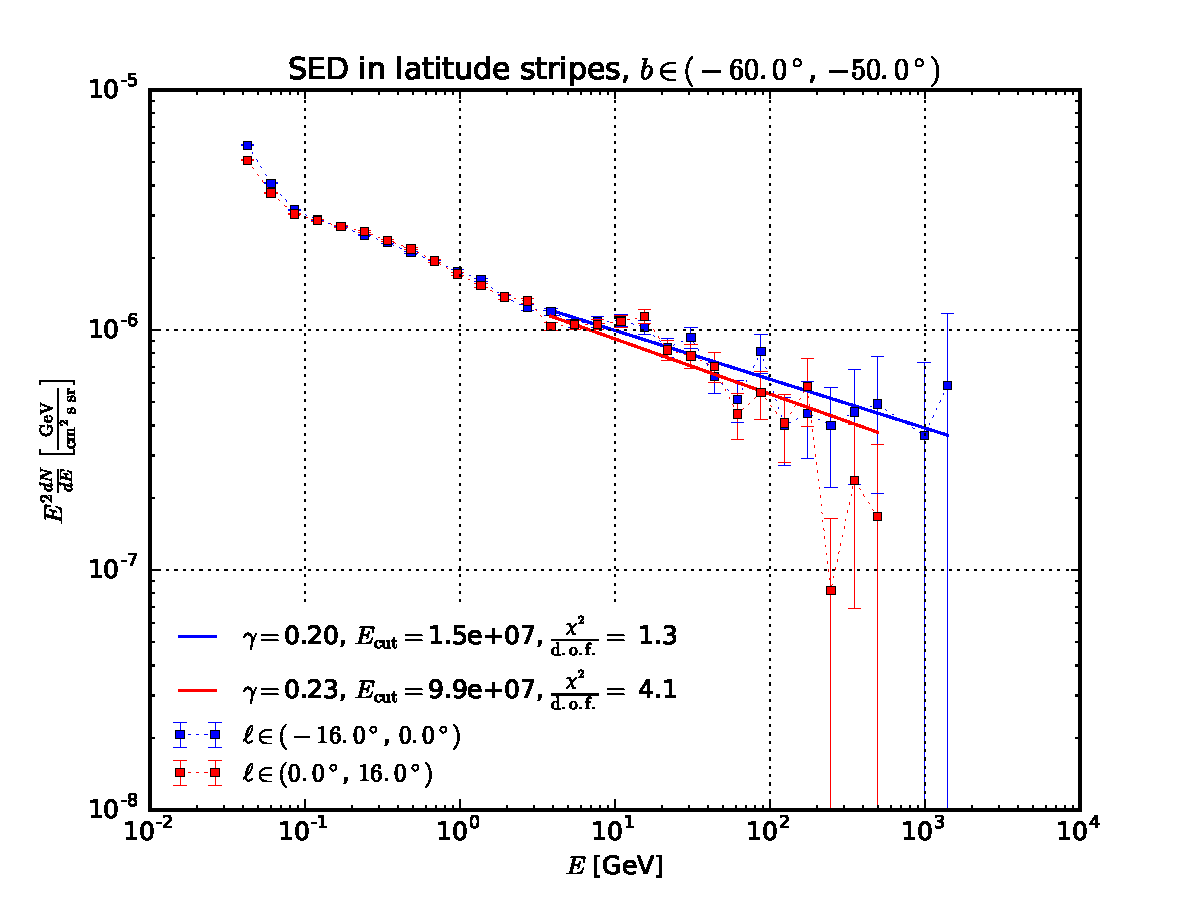
\includegraphics[width=\textwidth]{spectrum_of_bottom_bubble_in_lat_stripes_50-60.pdf}
    \end{subfigure}
    \caption{Same as above but for southern hemisphere. The spectrum of the eastern part of the south bubble lies slightly above the spectrum of the western part. The cocoon is there.}
\end{figure}


\begin{figure}
    \begin{subfigure}{0.5\textwidth}
        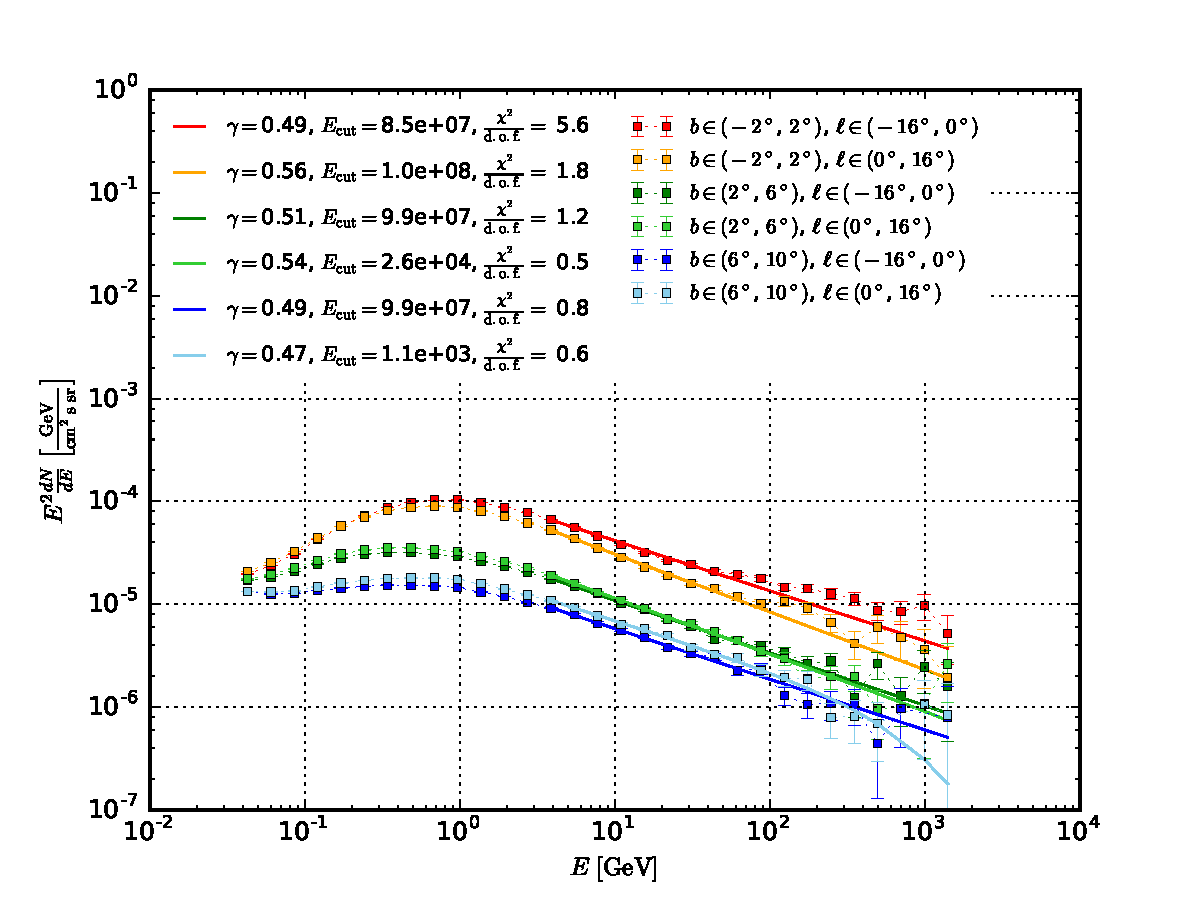
\includegraphics[width=\textwidth]{SED_top.pdf}
    \end{subfigure} 
    \begin{subfigure}{0.5\textwidth}
        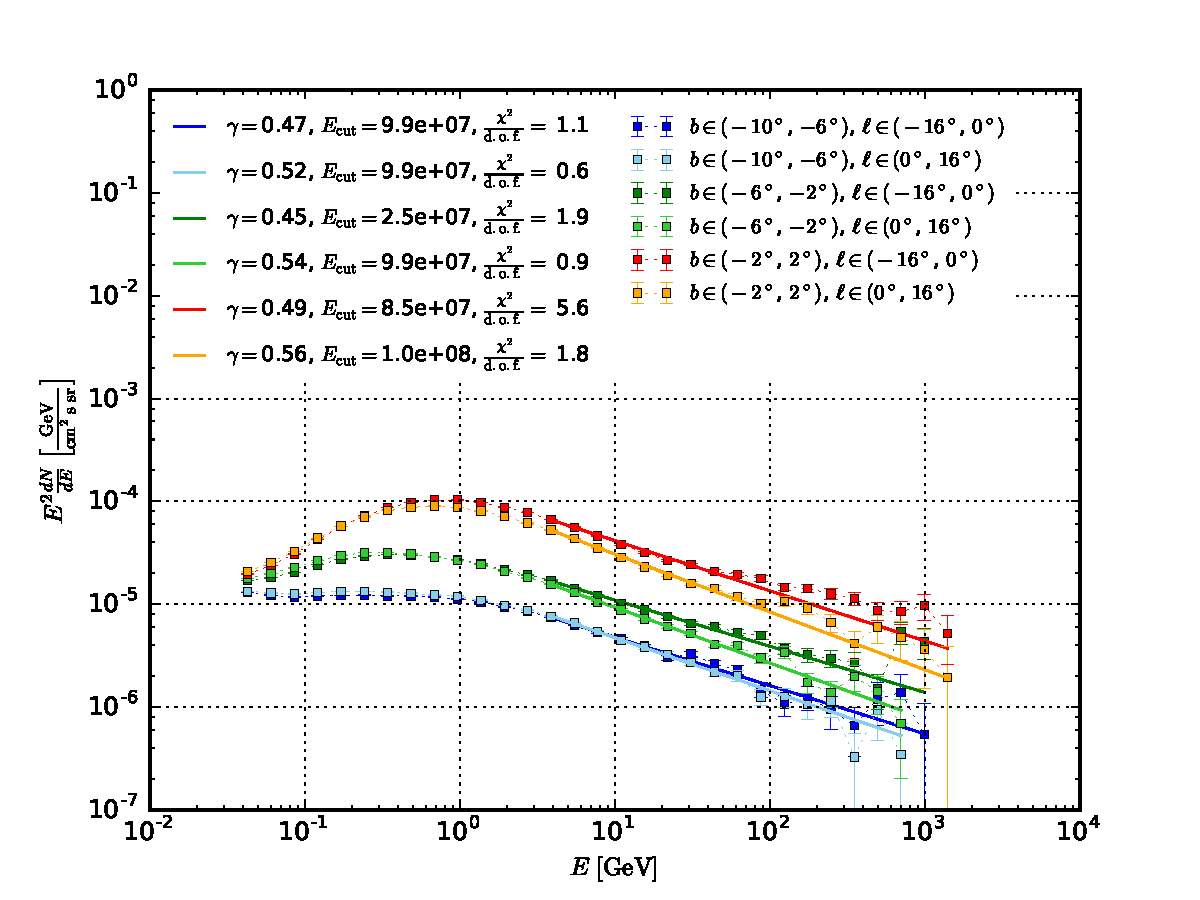
\includegraphics[width=\textwidth]{SED_bottom.pdf}
    \end{subfigure}
    \caption{SED at low latitudes of northern (left) and southern bubble (right). Point sources are masked. A powerlaw with cutoff is fitted to the spectra. Here at low latitudes the western regions have visibly harder spectra. This can also be seen very well in the residuals of the low-energy data model.}
\end{figure}

\begin{figure}
	\centering
    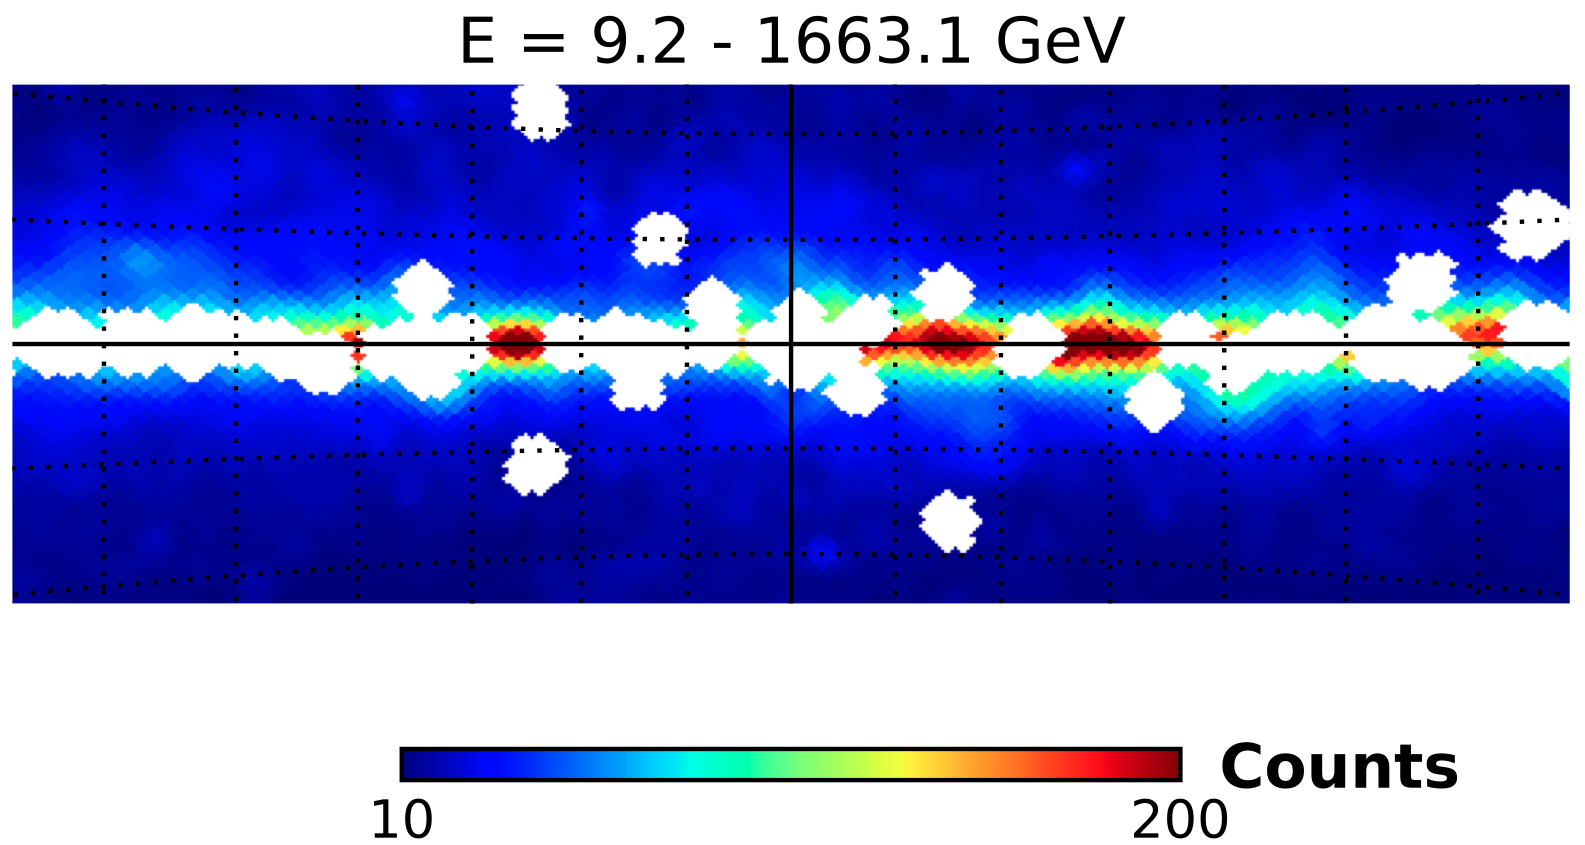
\includegraphics[width = 0.70\textwidth]{Gnomview9-1663GeV}
    \caption{Photon counts map in Gnomview. Point sources are masked (white circles).}
\end{figure} 

\end{document}
